\newpage

\chapter{Future Directions}

So far in this project, the work has primarily revolved around utilizing SPARTA to reproduce results of well-known physical phenomena. So far 1D and 2D phenomena have been reproduced with great accuracy. However, there are several new setups that can be explored. One such change would be to start utilizing \textbf{polyatomic molecules} instead of the monoatomic Argon that has been used so far. This is one of the true strengths of SPARTA as it's very difficult to obtain analytical solutions for such flow problems when considering polyatomic molecules due to the higher degrees of freedom available. Furthermore, 3D simulations can be performed, visualized, and compared with experimental data and can even be used to explain experimentally obtained results. \\

\no One idea that is interesting is to simulate the flow around a sphere in Martian conditions. This problem is particularly fascinating as it not only involves conditions where experiments are harder to be performed, but it also falls right in the strength of SPARTA as the atmosphere in Mars is far more rarefied than the atmosphere on Earth. The most abundant gas in the Martian atmosphere is carbon dioxide which is polyatomic. The temperatures and pressures vary quite a lot on Mars.  Lastly, there is also a growing interest in space expeditions to Mars, and such studies on the Martian atmosphere are filled with potential breakthroughs in our understanding of interplanetary expeditions. All these characteristic features of the Martian atmosphere problem put together make this a particularly interesting and promising area of research. Some data pertaining to the Martian atmosphere has been presented in the following section.

\section{Martian Atmosphere}

Mars has a very unique atmosphere. Unlike Earth's warm atmosphere, the temperatures on Mars lie predominantly between 166 K and 256 K, which is well below the freezing point of water at sea level. The atmosphere at Mars is also very thin, having a mean atmospheric pressure of about 600 Pa in comparison to Earth's 110,000 Pa. One feature that can be observed nowhere on Earth is the low thermal inertia that the Martian atmosphere possesses. Temperature swings of the order of 100 K can happen over short durations of time. There are also \textit{katabatic} winds on Mars, which are winds that are accelerated down a slope by gravity and a density gradient. These are similar to the katabatic winds found in some places like Greenland. Another feature that leads to some very interesting phenomena is the presence of atmospheric electricity on Mars. Some of these phenomena have been described by Rahman \textit{et al.} \cite{rahman2023turbulence}.

\subsection{Descent Characteristics}

Over here, the pressure, temperature, and density of the Martian atmosphere are described using the data obtained by NASA's Curiosity Rover from the Planetary Data System \cite{holstein2016atmospheric}. Figure \ref{gra:temp} shows the variation of atmospheric temperature with height.

\begin{figure}[H]
  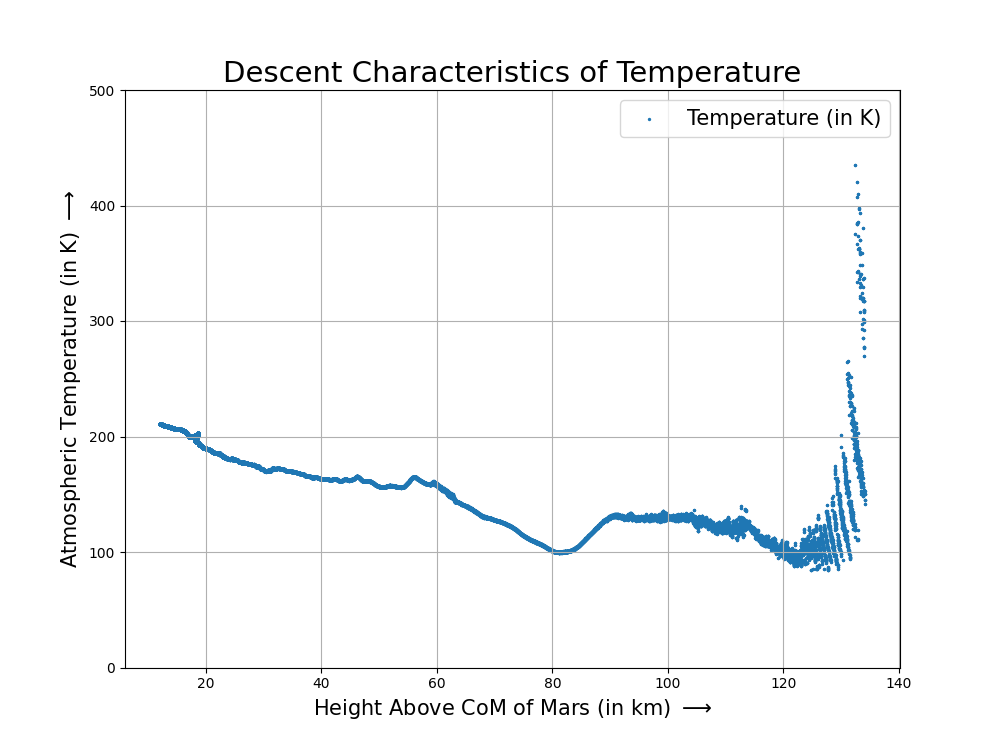
\includegraphics[scale=0.4]{Pictures/Chapter_7_Future/Cleaned_Temperature_Plot.png}
  \centering
  \caption{Variation of atmospheric temperature with height on Mars}
  \label{gra:temp}
\end{figure}

\no One can see that the temperature is high at the upper layers of the atmosphere, obtains a minima somewhere in between and again increases towards the surface of the planet. This can be attributed to a combination of solar radiation, the thermal radiation of the surface of Mars and, the low thermal conductivity of air. This variation is qualitatively similar to the variation on Earth, represented in Figure \ref{gra:temp_e}.

\begin{figure}[H]
	\centering
    \includesvg[width=0.65\linewidth]{Pictures/Chapter_7_Future/Temperature.svg}
    \caption{Variation of atmospheric temperature with height on Earth}
	\label{gra:temp_e}
\end{figure}

\no Figure \ref{gra:pres} shows the variation of atmospheric pressure with height. Notice how this decreasing linear profile on a logarithmic scale suggests an exponential decay in pressure, much like what is observed on Earth (Figure \ref{gra:pres_e}).

\begin{figure}[H]
  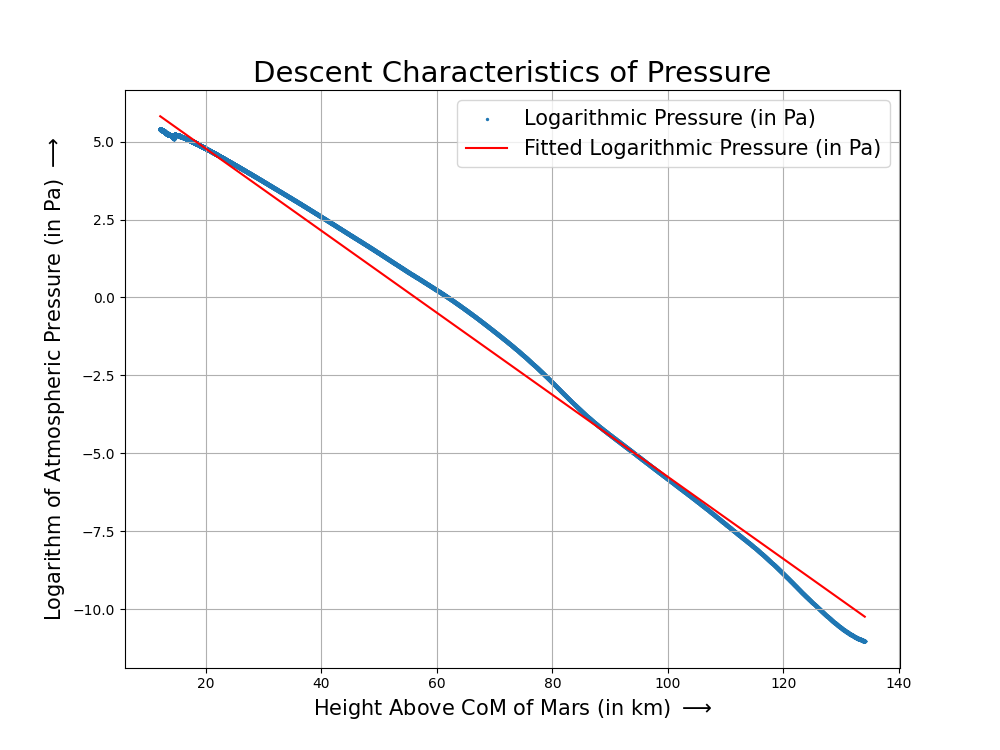
\includegraphics[scale=0.4]{Pictures/Chapter_7_Future/Log_Pressure_Plot.png}
  \centering
  \caption{Variation of atmospheric pressure with height on Mars}
  \label{gra:pres}
\end{figure}

\begin{figure}[H]
	\centering
    \includesvg[width=0.65\linewidth]{Pictures/Chapter_7_Future/Log_Pressure.svg}
    \caption{Variation of atmospheric pressure with height on Earth}
	\label{gra:pres_e}
\end{figure}

\no Figure \ref{gra:dens} shows the variation of atmospheric density with height. Notice how this decreasing linear profile on a logarithmic scale suggests an exponential decay in density, much like what is observed on Earth (Figure \ref{gra:dens_e}). This close qualitative matching of the properties of Earth and the Martian atmosphere is very interesting, implying only a scale difference between the two planets on a high level.

\begin{figure}[H]
  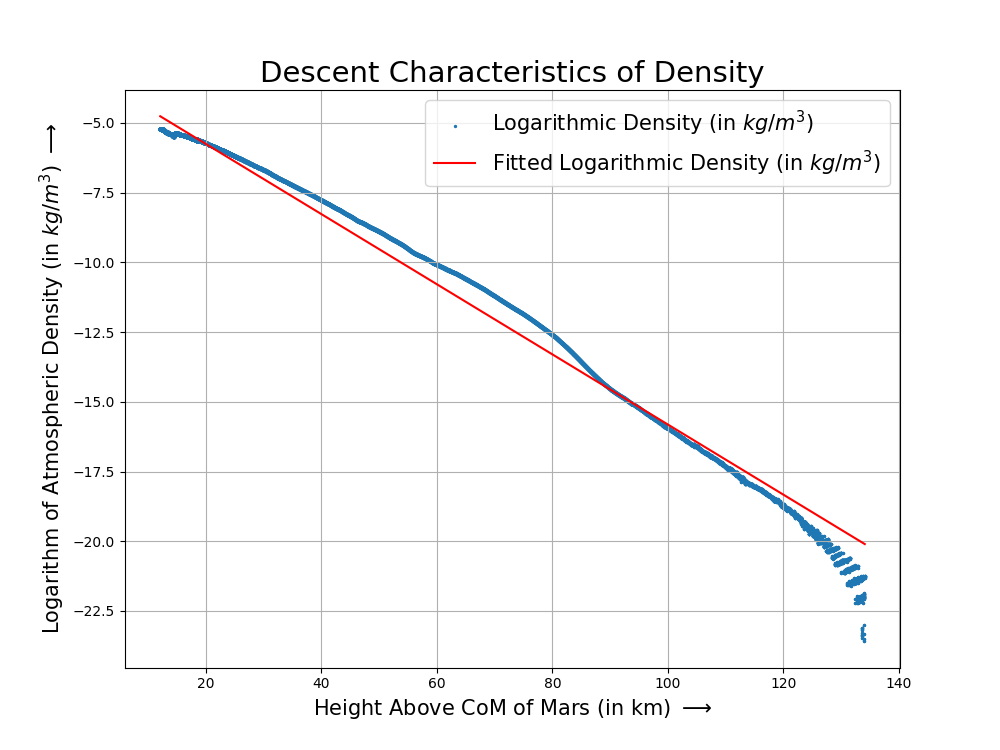
\includegraphics[scale=0.4]{Pictures/Chapter_7_Future/Log_Density_Plot.png}
  \centering
  \caption{Variation of atmospheric density with height on Mars}
  \label{gra:dens}
\end{figure}

\begin{figure}[H]
	\centering
    \includesvg[width=0.65\linewidth]{Pictures/Chapter_7_Future/Log_Density.svg}
    \caption{Variation of atmospheric density with height on Earth}
	\label{gra:dens_e}
\end{figure}

\subsection{Chemical Composition}

The chemical composition of Mars is quite different from that observed on Earth. Below, the data from a few experiments from the Mars Science Laboratory's Reduced Data Records (RDR) repository \cite{rdr2013mars} are plotted. Again, all of the plots, the code to scrape the data from RDR, and the plots are available in the repository containing this project \cite{Raghuveeran_Work_During_Summer_2024}.

\begin{figure}[H]
  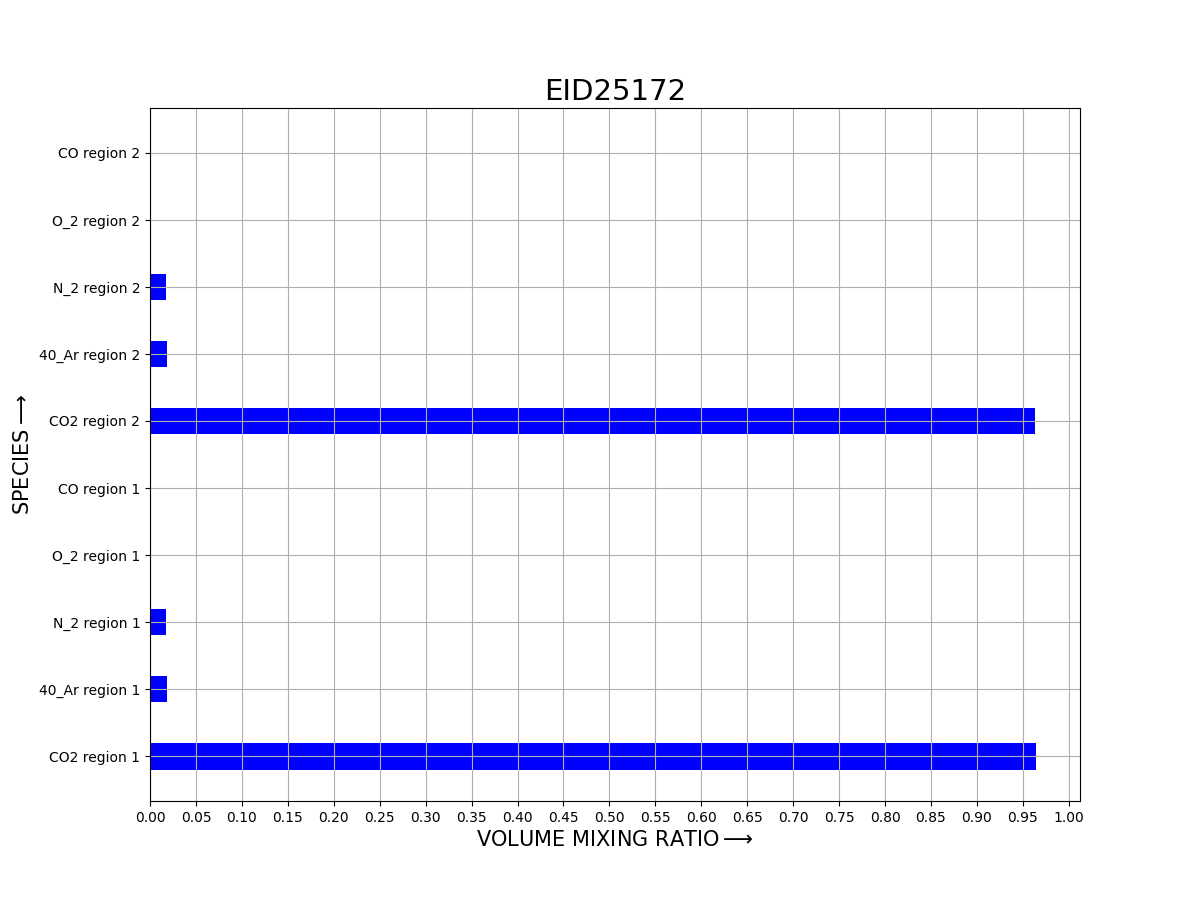
\includegraphics[scale=0.4]{Pictures/Chapter_7_Future/EID25172.png}
  \centering
  \caption{Relative abundance of compounds in the Martian atmophere}
  \label{gra:qms}
\end{figure}

\no The final data presented are the \textbf{volume mixing ratios} of various compounds in the Martian atmosphere obtained using the \textbf{Quadrupole Mass Spectrometer} (QMS) present on the Curiosity rover. Figure \ref{gra:qms} gives a representative plot of the data in RDR. From the plot, we can clearly infer that carbon dioxide is the most prominent gas in the Martian atmosphere, followed by nitrogen and argon.